\section{Results \& Statistical Analyses @ALL}
\subsection{Localizing sources linearly discriminating synchronous and asynchronous events based on ERPs}
% show ERPs at FCz/Pz and add significant differences between congruent and incongruent (across main effect haptics), show LDA pattern at window of peak differences in ERP, show weighted dipoles at peak differences in ERPs
% classification result

\begin{figure}{\textwidth}[h]
    \centering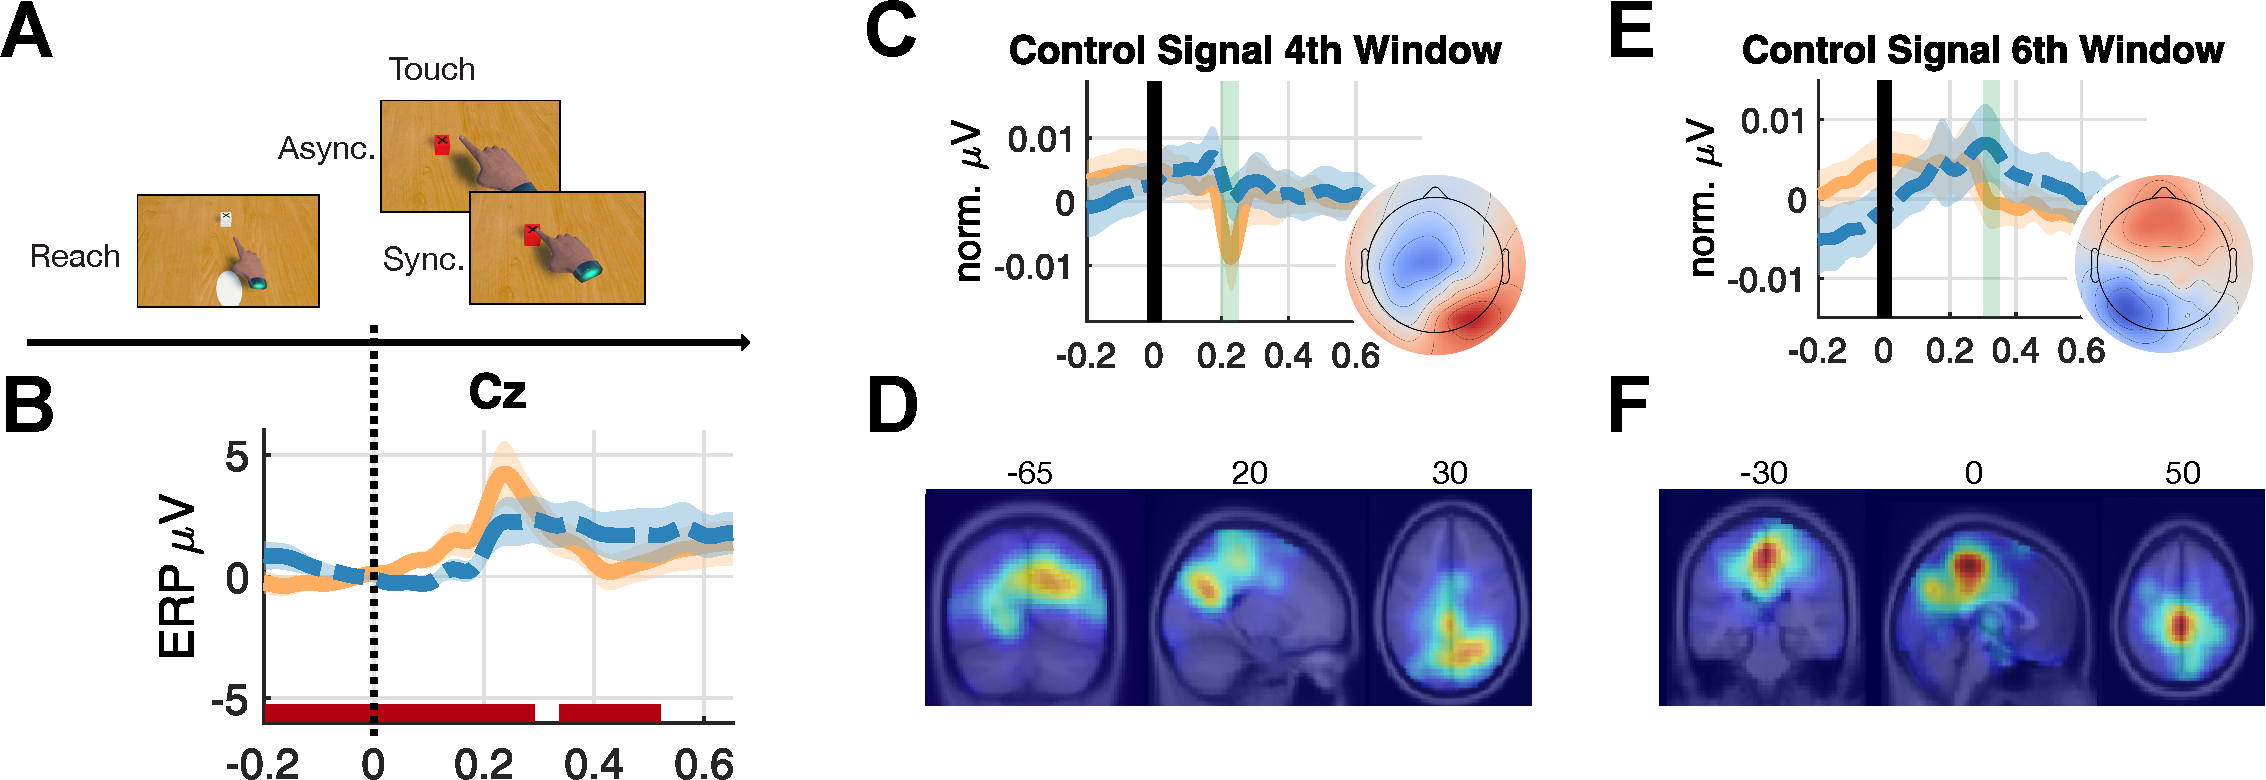
\includegraphics[width=\textwidth]{figures/fig1_lda/fig1_lda.pdf}
    \label{lda}
    \caption{Caption text 1}
\end{figure}

some buzzwords:
updating behavioral policy to 
visuomotor mapping
perturbation, i.e. a prediction error.

paper claim:
(touch epochs)
1. LDA location: Central-parietal EEG source activity discriminates between predicted and perturbed visuo-haptic perceptual experiences, in our case the touching of a cube on a desk, baring similarities to a classical simon task.

(full epochs)
2.1. ICs clustered to the centroid of the weighted ICs contributing the strongest to the LDA classifier were located to an area between precuneus and posterior cingulate cortex.
2.2. Hand velocity characteristics, an event-related potential as well as an event-related spectral signature were explained by adding a haptic channel, increasing the level of immersion in the perceptual experience.
2.3. Further, we observed responses locked to the feedback onset independent of differences in ongoing motor behavior between matching and mismatching classes. (description-level)

(touch epochs)
3.1. IC source dynamics following a visuo-haptic perturbation differ from predicted perceptual experiences (see 1., show difference erp and ersp)
3.2. Following a visuo-haptic perturbation, the context of said perturbation operationalized by hand velocity, haptic feedback and their interaction, impact IC source dynamics only faintly.

(next trial epochs)
4. Post perturbation behavioral adaptation is in line with previous findings and may be explainable through reinforcement learning like computations in the brain.

\begin{figure}{\textwidth}[h]
    \centering\includegraphics[width=\textwidth]{figures/fig2_overview_task/fig2_overview_task_small.pdf}
    \label{task}
    \caption{Caption text 1}
\end{figure}

Fazit:
Coherent multisensory integration yields meaningful perceptual experiences and is central to adaptive behavior because it allows animals to perceive a world of coherent perceptual entities. IC sources located near posterior cingulate cortex may anchor the self in the afforded reference frame, providing grounds for spatial predictions during ongoing perceptual experience.

%so there are 2 things participants do in the task: 
%1. they collide too early and immediately adapt hand movement and have mmn / frontal theta -> Prediction Error
%2. they do RL using PE signal and adapt subsequent behavior (trial after mismatch)

